% !TeX root = ../thesis.tex
% !TeX spellcheck = en_US

As mentioned in the introductory motivation, the task of the developed \term{hybrid routing algorithm} is to find optimal paths through open spaces between arbitrary source and destination locations.
Current routing approaches are either incapable of correctly reaching arbitrary locations (in the case of graph-based algorithms like A*) or do not allow the use of existing road edges and speedup techniques (for example in the continuous Dijkstra approach).
Additionally, none of the existing approaches uses both, the open spaces between obstacles and an existing road network.
Latter may still contain relevant information for pedestrian navigation, such as sidewalk information, surface conditions or access restrictions, and are therefore relevant for routing.

The resulting hybrid routing algorithm does not have these disadvantages and therefore offers a flexible and accurate routing.
This chapter covers the implemented algorithm's design to accomplish these tasks.
First, the overall context is presented, especially the requirements and constraints of the algorithm.
Second, details on the routing strategy and general design decisions are presented.
Finally, an overview of the separate components and a description of the deployment of this algorithm is given.

\section{Requirements and constraints}
	
	Enhancing the routing capabilities of the MARS framework is an integral aspect of this work.
	Even though the implementation is based on MARS, the overall design and the resulting architecture is independent of MARS.
	Integrating the algorithm into a different context or using it as a standalone application is therefore possible with no or minimal changes in the code.
	
	Apart from the integration into MARS, there are several requirements on the algorithm itself, which are presented in the following.
	Technical constraints also exist and are discussed at the end of this section.
	
	\subsection{Requirements}
	
		Functional requirements of the resulting software can be formulated without problems since this is not a complex software system but a single algorithm with a distinct task.
		The hybrid routing algorithm should determine an optimal path between two arbitrary locations by following existing ways but also by traversing open spaces while avoiding obstacles.
		An optional weight function should assign custom edge weights to find minimum-weight paths.
		The weight function should enable the algorithm to alternate between road segments and open spaces.
		
		More complex and time-consuming are the quality requirements.
		Because this is not part of a commercial software development, these requirements are not part of any specification.
		Nonetheless, they exist and consist of the following aspects.
	
		The most important quality requirement in terms of effort is performance.
		It affects large parts of the software architecture since the resulting algorithm, despite its complexity, should ideally have a negligible impact on the overall performance of a simulation compared to current graph-based routing approaches.
		Routing algorithms and engines often consist of a preprocessing and query-answering stage.
		In order to create fluent and fast simulations, the performance of answering numerous routing requests must be as good as possible.
		The time needed for preprocessing, however, is of less importance.
		
		The most essential requirement is the correctness of the resulting routes, meaning the algorithm must determine the truly minimum-weight paths according to a given weight function.
		Another quality requirement is the closeness of the resulting routes to actual pedestrian behavior.
		Unfortunately, this can hardly be measured without having extensive data of pedestrians and their actual tracks in the real world.
		Ideally, the trajectory of a calculated route should be identical to a real-world pedestrian track and should at least make sense to an outside observer.
		The trajectories of the shortest path and a real-world route should be as similar as possible.
		However, real pedestrian behavior, for example, keeping a minimum distance to obstacles, is not part of the shortest path calculations presented in this thesis, but rather a task of modeling a pedestrian agent.
	
	\subsection{Constraints}
	\label{subsec:constraints}
		
		One major constraint is the ability to integrate the implementation of the final algorithm into the \term*{MARS} framework.
		This means the programming language C\# and the use of the \term{NetTopologySuite} (\term*{NTS}) library are predetermined since MARS is based on these as well.
		However, these technical constraints do not affect the higher-level architecture and its components.
		
		The planned integration into another code base, in this case the one of the MARS framework, affects the management of dependencies.
		On the one hand, the amount of newly introduced dependencies should be kept to a minimum, which means dependencies on MARS and NTS are to be preferred over other third-party libraries.
		On the other hand, using only libraries on which MARS depends as well is not always possible due to version mismatches.
		More specifically, a triangulation method was needed, which is part of a more recent NTS version incompatible with MARS at the point of development.
		However, this case only appeared once, can easily be circumvented and should disappear with future dependency updates.
		
		An additional constraint is the limitation on vector data as the tape of geodata used for obstacles and roads.
		Using raster data is theoretically possible, as mentioned in \Cref{subsection:generate-graphs-from-maps} for the work of Walter et al., but requires additional and different processing steps.
		Therefore, only vector data is supported.
	
\section{Combination of routing algorithms}
\label{sec:combining-routing-algorithms}

	This section describes the core aspect of this thesis:
	The decision on a strategy to combine graph and geometric routing algorithms.
	A decision on this \enquote{merge} strategy is crucial to the design and architecture of the application.
	
	The following four approach candidates were considered and are discussed in the following.
	The last approach was considered the most promising and was therefore implemented.
	\begin{enumerate}
		\item Ad hoc generation of edges
		\item Concurrent routing
		\item Concurrent routing on smaller segments
		\item Merge of an existing network with a visibility graph
	\end{enumerate}
	
	\subsection{Ad hoc generation of edges}
	
		The idea of an ad hoc generation of edges is the following:
		Whenever the graph routing algorithm reaches a road junction, it is paused and the \term*[continuous Dijkstra paradigm]{continuous Dijkstra} algorithm is started.
		No destination vertex is defined, which means the geometric routing will be stopped after the furthest wavefront reaches a certain distance.
		The continuous Dijkstra approach creates a shortest path map, so the shortest paths to all reached vertices in the road graph are calculated.
		All shortest path edges are then added to the road graph and the paused graph-based routing resumes.
		A real-world example of this approach would be a pedestrian walking down a road, stopping at a junction and consulting a map to decide on which path to continue.
		
		The advantage of this approach is the realistic behavior of pedestrians not planning the entire route in beforehand.
		In fact, Teknomo and Millonig introduced a routing mechanism for agent-based simulations with the assumption of little to no apriori knowledge of agents about their environment\cite{teknomo-millonig-routing}.
		This approach would, therefore, partially implement their assumptions on an agent's behavior.
		
		One disadvantage is a relatively high complexity since no standard algorithm from software frameworks used in this work supports a pause functionality, so any existing routing algorithm would have to be manually adjusted.

		Also, this approach will likely cause performance issues.
		When using Dijkstra as a graph-based routing algorithm, $\bigo{|V|}$ many vertices are visited, causing $\bigo{|V|}$ many geometric routing queries for the continuous Dijkstra algorithm.
		Even when using the algorithm from Hershberger and Suri\cite{hershberger-suri} with a time complexity of $\bigo{n \log n}$, it can be assumed that $n > |V|$ resulting in a complexity of $\omega(|V|^2)$.
		Caching the shortest path map using a \term*{CPD} would increase query performance but it would also increase implementation complexity and processing time during preprocessing.
		Instead, precomputing all shortest path edges and directly merging them into the road graph would eliminate complexities, enhance performance and is used in the fourth approach.
		
		The ad hoc idea of this approach yields no significant advantage compared to a preprocessing-based algorithm.
		Therefore, this approach was not further pursued.
	
	\subsection{Concurrent routing}
	
		Combining the results of two concurrent routing procedures, one graph-based and one geometric, is another approach.
		Splitting the resulting paths at intersection points and only choosing minimum-weight segments yields the overall shortest path, which potentially alternates between graph-based segments and segments from geometric routing.
		
		The most prominent advantage is the simplicity of answering routing requests since known routing algorithms could be used.
		Therefore, it would be relatively easy to implement and speedup techniques could be used for the graph-based routing.
		
		However, there are two significant disadvantages.
		First, it is uncertain whether the two paths are actually intersecting at any point.
		Second, even if they do intersecting, too few intersections on a long route result in suboptimal paths because routing parts of a long segment with the respective other routing technique might further reduce the overall weight.
		Only if two routes intersect frequently enough, the selection of segments based on the weight function could result in good routes.
	
	\subsection{Concurrent routing on smaller segments}
	
		This approach is very similar to the one above, but it tries to fix the uncertainty of intersections between the two resulting paths.
		Multiple ways are conceivable to ensure enough intersections exist or to otherwise guarantee that segments are small enough to be merged.
		
		One way is to stop the two routing algorithms after a certain distance at the next available vertex.
		After stopping for the first time, there are two such end vertices, one where the graph-based and one where the geometric routing stopped.
		From each vertex, two new routing queries start and stop again after a certain distance resulting in four new end vertices.
		This continues until one query reaches the destination.
		On the one hand, this yields arbitrarily small segments for later merging, but on the other hand, this results in $\bigo{2^n}$ many routing queries with $n$ segments in the overall shortest path.
		Even though each query is short, this approach would not scale very well even with the help of heuristics or other helping mechanisms.
		
		A different approach to obtain smaller segments would be the following:
		First, the shortest path on the road graph is determined and split into segments of specific length connecting the vertices $v_0, v_1, ..., v_n$ with $v_n$ being the destination.
		Geometric shortest paths are determined between all points, resulting in $O(n^2)$ many routing queries.
		The graph-based segments and the geometric routing results are then merged, forming a new intermediate graph.
		Finally, one last routing query on this intermediate graph is performed to get the final optimal route.
		Other combinatorial approaches could be used instead of an intermediate graph since the shortest path problem is a combinatorial problem and, thus, can be solved using linear programming\cite{handler-zang-lp-duality}.
		
		There are likely to be more possible ways to ensure a sufficient amount of segments or intersections.
		However, this overall approach was not further pursued because both approaches have worse time complexities than any popular routing algorithm, including pure geometric routing.
		The first one would cause $\bigo{2^n}$ and the second one $\bigo{n^2}$ many routing requests, of which each request has a certain complexity itself.
		Even though the second idea might work well for appropriate segment lengths, the complexity and definite time overhead make it an unfavorable choice.
	
	\subsection{Merge of an existing network with a visibility graph}
	\label{subsec:design-merge-road-network}
	
		Previous approaches tried first to calculate shortest paths and then merge their results.
		This last approach, which was ultimately implemented, first merges a generated \term*{visibility graph} with an existing road graph.
		The actual merge operation is rather simple:
		Whenever a road edge and a visibility edge intersect, split the edges, create a new vertex at the intersection point and connect the split edges accordingly.
		
		Even though this approach is simple, the main disadvantage is the graph size.
		A visibility graph has $\bigo{|V|^2}$ many edges, which negatively affects the routing performance.
		
		Another disadvantage is the time complexity of the merge operation.
		All edges must be considered and, depending on the number of intersections, edges might be processed multiple times.
		This leads to at most $|E_R| \cdot |E_V|$ many merge operations for the routing graph edges $E_R$ and visibility edges $E_V$, which is in $\bigo{|E|^2}$ given all edges $E$.
		
		Fortunately, road networks are very sparse and often have a vertex degree between three and six\cite{zhao-analysis-osm-bejing}\cite{boeing-osmnx}, resulting in a probably much better runtime behavior in practice.
		An analysis of OpenStreetMap data for the road network of Germany's densely populated states North Rhine-Westphalia (NRW) and Hamburg (HH) showed node degrees of 3.1 (NRW) and 3.11 (HH).
		A vertex with a degree of 10 or higher did not exist in either of these states.
		
		Despite the disadvantages of this approach, I considered the advantages to be more important.
		As already mentioned, this strategy is not only simple, it also allows the use of speedup methods for routing queries (as presented in \Cref{subsec:speedup-methods}) and has potential for a wide range of performance optimizations as outlined in \Cref{sec:future-work}.
		Moreover, the resulting path is optimal based on the given weight function due to the usage of visibility edges, which are the shortest possible connections between vertices. 
		Also, no complex postprocessing and only one routing algorithm is needed.
		
		Taken all aspects into account, this strategy seemed to be the simplest and most promising with the least significant disadvantages.
		It was therefore chosen to be implemented.

\section{Design decisions}
\label{sec:design-decisions}

	Several design decisions were made after the decision of the strategy to combine graph-based and geometric routing fell.
	Some decisions did not influence the overall architecture and were just made to enhance performance or simplify the implementation, which are therefore described in \Cref{chap:implementation}.
	This section solely covers fundamental decisions relevant to the overall architecture.
	
	In this work, I implemented the visibility graph without using algorithms presented in the corresponding \hyperref[subsec:related-work:visibility-graph]{related work section}.
	None of the existing approaches would have been easy to implement without problems.
	Details on these problems and the exact reasons that led to the decision of a custom implementation are also presented in this section.
	
	\subsection{Requirements and considerations for the visibility graph creation}
	
		One essential requirement for the visibility graph creation is the ability to work with arbitrary obstacles, which primarily includes the fundamental point, linestring and polygon geometries.
		However, real-world datasets also contain multi-geometries such as multipolygons.
		Furthermore, assumptions about the collinearity, position of obstacles and intersections between them cannot be made for real-world datasets.
		
		An important special case arises for linestring obstacles with more than two vertices.
		Simply determining visibility edges to and from both sides of the linestring would result in shortest paths leading right through it because vertices of linestrings are visible from both sides.
		The same situation would arise with two arbitrary obstacles, including polygonal ones, touching each other in a single vertex.
		Both cases must be considered to ensure that shortest paths lead \emph{around} the obstacle.
		
		A core aspect of the routing algorithm is the reachability of arbitrary locations not represented by vertices within the graph.
		Therefore, adding visibility edges after the graph creation must be possible and should ideally be independent of the algorithm chosen to generate the graph and edges.
		
		As the generation of the routing graph happens in a preprocessing step, the time and space needed for this task was not a critical aspect of the whole algorithm.
		Further optimizations are possible and discussed in \Cref{sec:future-work}.
		The routing behavior is significant to agent-based simulations as it directly affects the time required for a simulation.
		Creating the graph in a preprocessing step decouples its processing time from the simulation, especially when persisting the graph for later uses.
		
		All these requirements and considerations, including problems and efforts outlined below, led to the decision of implementing a simple graph generation approach with some easy but effective optimizations.
	
	\subsection{Suitability of existing approaches}
	\label{subsec:suitablilty-edge-creation-approaches}

		The largest and most influential design decision was the decision against an approach from the literature as presented in \Cref{subsec:related-work:visibility-graph}.
		Several approaches from the literature have either restrictions on the geometric structures or assume that a certain preprocessing of the data has already been performed.
		
		The approach by Welzl\cite{welzl-visibility-graph}, for example, explicitly assumes that there are no collinear vertices, i.e. three or more vertices in a straight line.
		It may seem unlikely to occur in real-world datasets, but it is a common practice in OpenStreetMap to align touching buildings and other straight obstacles like walls.
		
		The optimized approach by Overmars and Welzl\cite{overmars-weizl-visibility-graph} only works on non-intersecting line segments.
		However, real-world data is too diverse to fulfill this criterion as polygons, longer linestrings and other more complex data structures exist.
		Splitting all geometries into such non-intersecting line segments would increase complexity and would also introduce new problems to solve.
		For example, splitting a polygon into line segments would require metadata on these segments to reconstruct the former polygon membership in order to avoid visibility edges within the former polygon, which would be created for an actual chain of linestrings.
		Handling all those special cases, preventing unwanted edges and still using the approach by Overmars and Welzl would be possible but significantly increases the complexity of their approach.
		
		Another approach with the limitation of no collinear vertices is the plane-sweep algorithm by Ghosh and Mount\cite{ghosh-output-sensitive-vgraph}.
		In addition to the limitation on collinear vertices, they assume x-coordinates to be unique, which would need to be handled as well.
		Even though coordinates are usually floating point numbers and therefore have a great range of possible values, rounding and size limitations reduce this range and might result in a high number of non-unique x-coordinate values.
		Counting the number of non-unique x-coordinates in OpenStreetMap illustrates this problem:
		Of all coordinates in the OSM dataset of the German state of Hamburg, 22.8\% are non-unique.
		
		Kapoor and Maheshwari presented a visibility graph creation as well\cite{kapoor-shortest-path-vgraph} but assumed a triangulation of the open space between the obstacles.
		Such a triangulation can be done relatively fast, algorithms with time complexities of $\bigo{n \log{n}}$ and better are known\cite[58-60]{de-berg-computational-geometry}.
		However, libraries such as MARS or the NetTopologySuite do not support triangulation for open spaces, only for closed geometries.
		Implementing an algorithm for this task would be needed in addition to the visibility graph creation algorithm.
		
		All approaches from the literature would probably work but preprocessing, restrictions on the input data or adjustments to the approaches would be necessary.
		Since this work focuses more on the overall concept of a hybrid routing algorithm, the choice of the graph generation algorithm was less important to me.
		Therefore, the implementation in this work, as shown in \Cref{chap:implementation} in detail, is simpler and independent of the aforementioned approaches.
		
	\subsection{Early implementation based on the continuous Dijkstra paradigm}
		
		Before the decision for a routing strategy fell, a prototype implementation was created based on the \term*{continuous Dijkstra paradigm} with propagating wavefronts.
		However, next to the overall strategy decision on the visibility graph approach, two additional reasons existed for a visibility graph-based algorithm.
		
		One reason was the implementation of performance enhancement for the continuous Dijkstra algorithm.
		Early stages used a very naive and simple implementation without optimizations mentioned in recent literature on this topic.
		Wavefronts did not move continuously, but instead, they \enquote{snapped} to the next event, i.e. to the next collision with a visible vertex where new wavelets can spawn.
		In this early implementation, no extensive efforts went into optimizations, e.g. by implementing the approach presented by Hershberger and Suri\cite{hershberger-suri}.
		Instead, a simple preprocessing was introduced, which led to a significant performance improvement.
		Because a wavefront only reaches vertices visible to the origin of the wavefront (which is vertes itself), the visibility between all vertices was determined and used for the events mentioned above.
		Such predetermined visibilities are the core idea of a visibility graph, thus, moving to an approach using an actual visibility graph was only a small step.
		
		A second reason against this early continuous Dijkstra implementation was the difficulties and the disadvantages of combining the network-based routing with the continuous Dijkstra algorithm, as described in \Cref{sec:combining-routing-algorithms}.
		
		Therefore, this first continuous Dijkstra approach was not further pursued but converted to a generator for a routable visibility graph with components described in the following section.
	
\section{Components}
\label{sec:components}

	The hybrid routing algorithm consists of two main components presenting public interfaces.
	Generating the underlying routing graph, the so-called \term{hybrid visibility graph}, is the first step and resides in its own component, the \texttt{HybridVisibilityGraphGenerator} class.
	The hybrid visibility graph itself is contained in the \texttt{HybridVisibilityGraph} class, which primarily contains the graph structure and is used to answer routing queries.
	A third but internal component, not intended to be used from outside the algorithm, is the \texttt{VisibilityGraphGenerator}, which creates the visibility edges for the routable hybrid visibility graph.
	Since this work resides in a rather technical and algorithmically oriented context, no other components are involved, such as a user interface, application server or database.
	
	\begin{figure}[h]
		\begin{figcenter}
			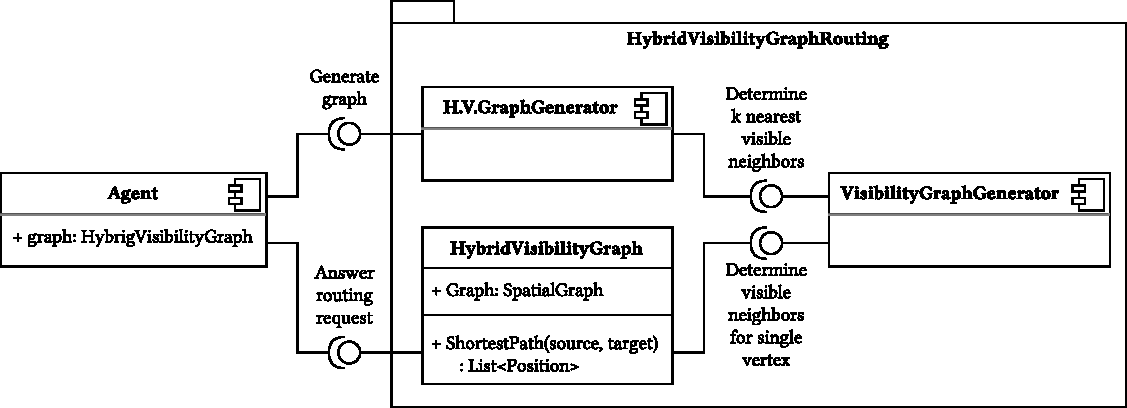
\includegraphics[scale=0.8]{images/components.pdf}
		\end{figcenter}
		\caption[Component diagram of the hybrid visibility graph implementation.]{The components and usages of interfaces of the resulting implementation.}
		\label{fig:components}
	\end{figure}
	
	\begin{figure}[h]
		\begin{figcenter}
			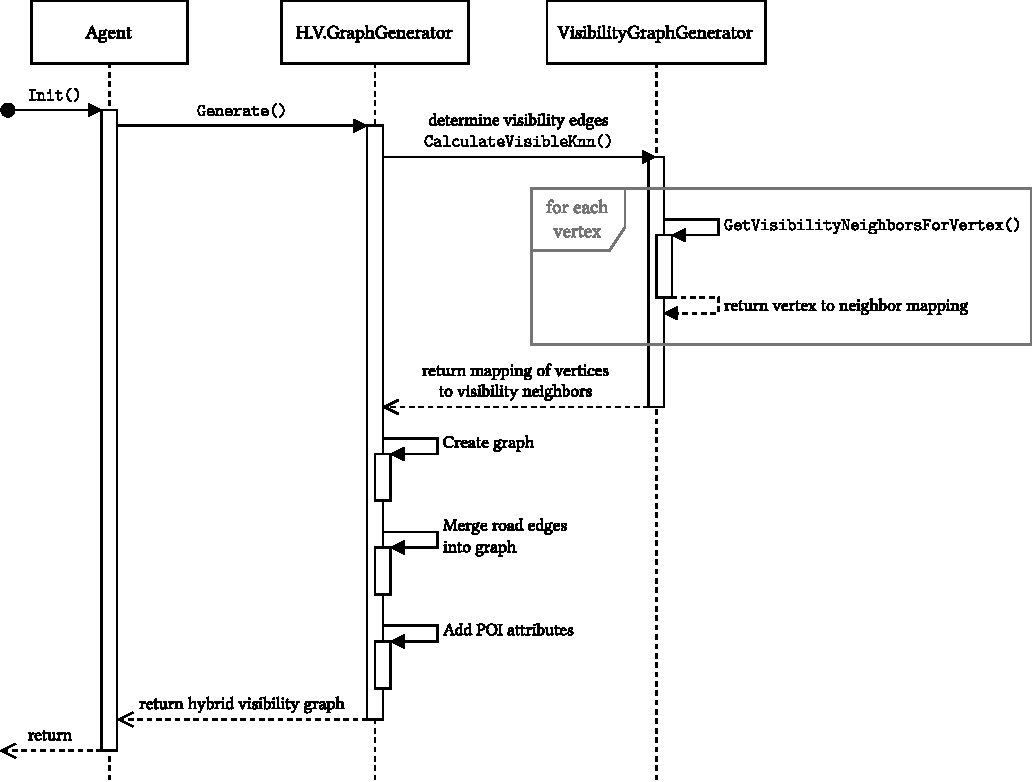
\includegraphics[scale=0.8]{images/components-sequence-generation.pdf}
		\end{figcenter}
		\caption[Sequence-diagram of hybrid visibility graph generation.]{The generation process to obtain the hybrid visibility graph.}
		\label{fig:components-sequence-generate}
		\hfill
		\\
		\begin{figcenter}
			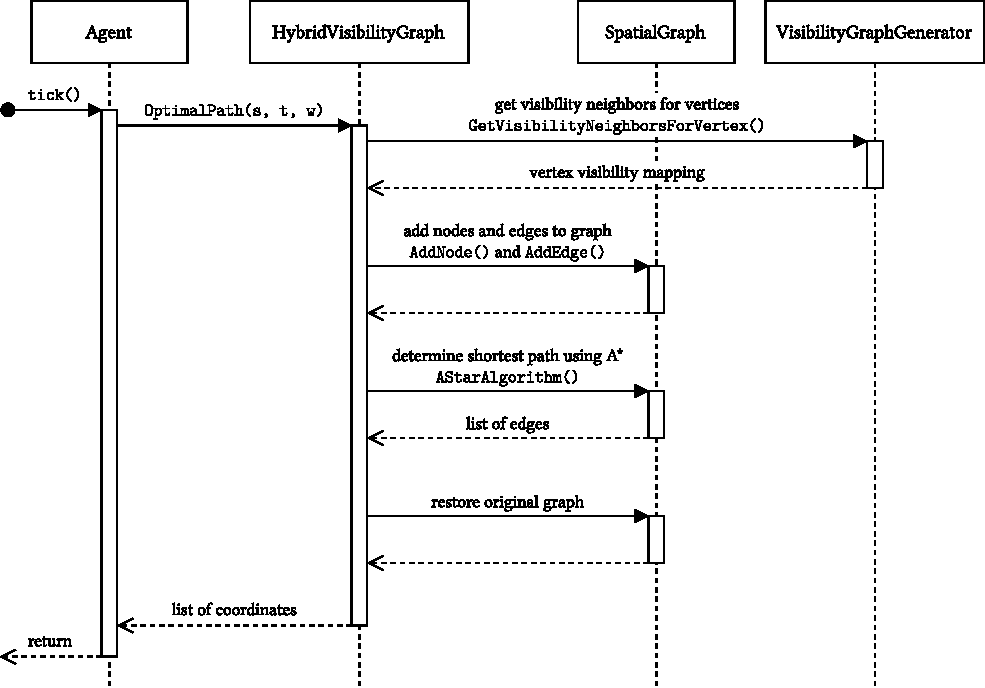
\includegraphics[scale=0.8]{images/components-sequence-routing.pdf}
		\end{figcenter}
		\caption[Sequence-diagram of routing queries.]{The most important steps performed during a routing request using the hybrid visibility graph. The variables \texttt{s}, \texttt{t} and \texttt{w} are the source vertex, the target vertex and the weight function.}
		\label{fig:components-sequence-routing}
	\end{figure}
	
	In an agent-based simulation, determining routes is part of the agent's path-planning routine.
	The hybrid visibility graph has the necessary interfaces to answer routing queries, meaning an agent needs access to an instance of this graph.
	\Cref{fig:components} illustrates this with an exemplary agent holding an instance of the hybrid visibility graph, which can be created once and shared among multiple agents.
	
	The \texttt{HybridVisibilityGraphGenerator} (abbreviated as \enquote{H.V.GraphGenerator} in \Cref{fig:components-sequence-generate}) presents a public \texttt{Generate()} method for the task of the graph generation and, in this exemplary setup, is used by the agent.
	It returns an instance of the \texttt{HybridVisibilityGraph} class offering public methods to answer shortest path queries.
	\Cref{fig:components-sequence-routing} illustrates the internal tasks of a routing request using the \texttt{OptimalPath(source, destination, weightFunction)} query method.
	The result is a list of coordinates representing the shortest path between two input coordinates.
	
	To fulfill the overall goal of this work of finding optimal paths between arbitrary locations, it must be ensured that these locations are reachable via the hybrid visibility graph.
	Without further consideration of the source and destination locations, there is no guarantee that these locations are represented by any vertex in the graph.
	Therefore, the hybrid visibility graph has to temporarily connect these locations to the graph if they are not present already.
	This is done by determining all visible neighbors of the source and destination locations and merging the resulting edges into the underlying graph.
	Because this is the same step performed during graph creation, the \texttt{VisibilityGraphGenerator} is used during routing as well to determine visibility neighbors of a single vertex.
	\Cref{sec:answering-queries} covers the process of answering routing queries in more detail, including a clean-up step that is performed after the shortest path has been found.
	
	The shortest path algorithm used is A*, which uses the underlying spatial graph of the hybrid visibility graph, which temporarily contains the additional edges to and from the source and destination vertices.
	A custom weight function allows exact control on how strong to prefer road edges.
	The effects of different weightings are evaluated in \Cref{subsubsec:manual-route-analysis}.

\section{Deployment}

	The goal of this thesis is to enhance route quality for agent-based simulations.
	Therefore, the algorithm was implemented using the MARS framework.
	In order to use this work to improve MARS, the code is published on GitHub\footnote{\url{https://github.com/hauke96/master-thesis/}}.
	The C\#-Project \enquote{HybridVisibilityGraphRouting} contains all necessary classes and interfaces, only the \texttt{Triangulation} project will be needed as well due to the aforementioned version mismatch regarding the triangulation of polygons.